
  \subsection{Programação Dinâmica}

    Programação dinâmica é um método para a construção de algoritmos para a resolução
    de problemas computacionais, em especial os de otimização combinatória.
    Ela é aplicável a problemas nos quais a solução ótima pode ser computada a 
    partir da solução ótima previamente calculada e memorizada - de forma a evitar recálculo - 
    de outros subproblemas que, sobrepostos, compõem o problema original.

    O que um problema de otimização deve ter para que a programação dinâmica 
    seja aplicável são duas principais características: subestrutura ótima e 
    superposição de subproblemas. Um problema apresenta uma subestrutura ótima 
    quando uma solução ótima para o problema contém em seu interior soluções 
    ótimas para subproblemas. A superposição de subproblemas acontece quando 
    um algoritmo recursivo reexamina o mesmo problema muitas vezes. 

    \subsubsection{Fibonnaci}

    \begin{figure}[ht]
      \centering
      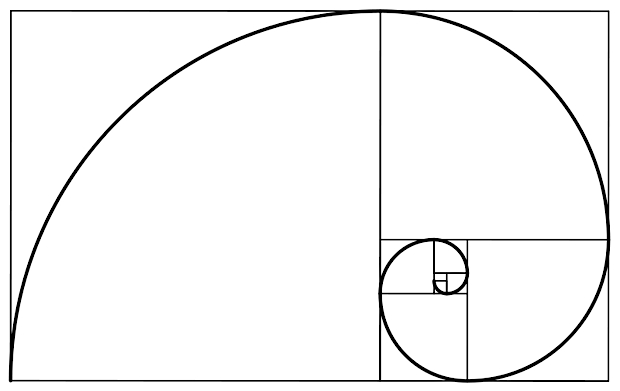
\includegraphics[width=.3\textwidth]{fibonnaci.jpg}
      \caption{Uma imagem ilustrativa da sequência Fibonnaci}
      \label{fig:fibonnaci}
    \end{figure}
